\chapter{Trabalhos Relacionados}

Nesse capítulo será apresentado alguns trabalhos em torno do tópico de desenvolvimento
de protocolos para rádios LoRa. Será feita um breve descrição dos trabalhos existentes,
uma explicação dos critérios que serão considerados ao comparar os projetos, e por fim, a
análise comparativa em si.

\section{LoRaCTP}

Lora Content Transfer Protocol, ou como chamado pelos criadores de LoRaCTP, é um 
protocolo baseado em LoRa para a transferência do que eles chamam de "conteúdos" entre dispositivos LoRa de maneira confiável, no sentido em que todos os dados que saírem do
remetente chegarão no destinatário. O projeto foi publicado em 2020 por K. Nakamura, P. Manzoni, M. Zennaro, J. -C. Cano e C. T. Calafate, 4 membros da Universidade Politécnica de Valência na 
Espanha e 1 membro do Centro Internacional de Física Teórica na Itália. O trabalho teve
como objetivo implementar um protocolo em cima da camada LoRa para a transferência de "conteúdos", que são simplesmente qualquer dado arbitrário de diferentes tamanhos, entre dois dispositivos com um rádio LoRa. Para atingir esse objetivo o protocolo divide o
conteúdo a ser envido em N pacotes, cada um com um tamanho fixo e 
abaixo do limite máximo que a modulação LoRa suporta. Cada um desses pacotes é encapsulado com um cabeçalho de 20 bytes, com informações do endereço do remetente, endereço do destinatário, flags e checksum. Para garantir o objetivo principal que é a entrega
de todos os pacotes ao destinatário, o protocolo segue a metodologia "stop-and-wait"
onde é enviado um pacote, e o próximo da sequência só será enviado após uma confirmação de
recebimento do destinatário dentro de 5 segundos. Os pacotes dessa forma devem ser enviados na ordem correta e no caso de falha de algum envio é feita no máximo 3 tentativas de 
retransmissão até ser considerado que existe algum problema no canal como ruído ou simplesmente ocupado, e a tentativa de envio do conteúdo é dada como falha. Entretanto o 
trabalho não entra em detalhes sobre o fluxo completo da transmissão dos dados, como se 
existe algum handshake antes da transmissão, e que metadados são trocados nesse handshake. LoRaCTP em teoria aceita conteúdos de tamanho ilimitados, mas no trabalho foi testado
conteúdos de até 150 Kbytes a uma distância de até 6 Km. O hardware utilizado para os testes
foi um LoPy4, uma placa de desenvolvimento embarcado com MicroPython e suporte para 4 diferentes tectonologias de rádio, LoRa, SigFox, WiFi e Bluetooth. O protocolo foi desenvolvido na linguagem Python e aberto ao público no Github. \cite{9394317}

\newpage

\section{LoRaMesher}

\begin{figure}[H]
    \centering
	\caption{LoRaMesher: ESP32 com LoRa numa rede Mesh}
    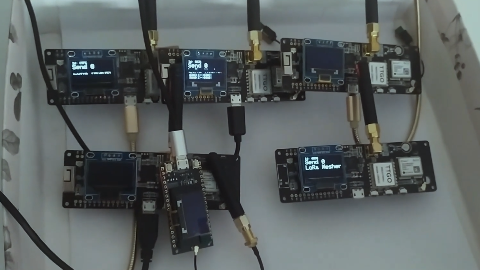
\includegraphics[width=0.6\textwidth]{img/loramesher.png}
    \label{fig:loramesher}
    
    Fonte: Implementation of a LoRa Mesh Library, 2022.
\end{figure}

Em outubro de 2022, Joan Miquel Solé, Roger Pueyo Centelles, Felix Freitag e Roc Meseguer publicaram
pela IEEE um trabalho chamado de "Implementation of a LoRa Mesh Library". A principal motivação dos
pesquisadores foi em notar que grande maioria das aplicações IoT com LoRa usam a arquitetura LoRaWAN
que possui limitações, como a de Nós finais da arquitetura não poderem se comunicar diretamente entre si mesmo quando a tecnologia LoRa fornece esse total suporte. Com isso, o objetivo principal dos
pesquisadores foi desenvolver uma arquitetura de rede alternativa ao LoRaWAN para dispositivos IoT
que melhor utilize os recursos da tecnologia LoRa. Os pesquisadores derem o nome para a implementação
de "LoRaMesher", uma biblioteca escrita em C++ desenvolvida para o microcontrolador ESP32 com chip LoRa
integrado. A biblioteca implementa uma topologia de rede Mesh e utiliza de APIs do FreeRTOS para
gerenciar recursos de memorias e processamento necessários para o protocolo. Foi implementado uma
metologia de transmissão confiável parecida com o "stop-and-wait" porém o protocolo é capaz de
calcular um tempo aproximado para que cada pacote de dado chegue no seu destinatário. Além disso foi
implementado um mecanismo de tratamento de colisão baseado no CSMA/CA, onde cada Nó primeiro verifica
se o canal está livre, para tentar utiliza-ló. A biblioteca tem código aberto e está disponível no Github para contribuição e uso, além disso ela possui uma pequena pagina Wiki para ajudar desenvolvedores que estão começando a utiliza-lá. No geral, o LoRaMesher é uma boa alternativa
para desenvolvedores IoT que precisam de mais flexibilidades de Rede no qual o LoRaWAN não suporta.
Pórem o LoraMesher pode apenas ser utilizado em microcontroladores IoT ESP32 com chip LoRa integrado,
além de que não tem implementado nenhum processo de empacotamento dos dados, implicando que se o
desenvolvedor necessita mandar mensagens maiores do que o payload do LoRaMesher suporta, ele
mesmo terá que implementar seu mecanismo de quebra de mensagens e empacotamento por cima do
LoRaMesher. \cite{9930341}

\newpage

\section{Critérios Comparativos}

Nesse capítulo foram escolhidos algumas características que serão levadas em consideração ao se comparar os trabalhos apresentados aqui. Nessa seção será apresentados esses critérios e suas descrições.

\begin{itemize}
    \item \textbf{Topologia de Rede:} A topologia de rede define de que forma os elementos de uma rede
    estão organizados, quais nós estão interligados e quais não estão, com isso surge diferentes possibilidades e também limitações para os fluxo de dados entre os participantes da rede. Segue algumas topologias existentes: Estrela, Mesh, Anel, Barramento, Estrela de Estrelas.
    \item \textbf{Transmissão Confiável:} Transmissão confiável é a existência de qualquer processo que
    garanta ou tente garantir que todos os dados enviados pelo destinatário chegaram no remetente. Um exemplo clássico são os protocolos da camada de transporte TCP e UDP, onde o TCP possui mecanismos de verificação se um pacote chegou no remetente, mas já o UDP simplesmente envia o pacote sem mecanismo algum de saber se ele foi recebido ou não.
    \item \textbf{Tratamento de Colisão:} Independente do canal de comunicação, sempre haverá uma limitação em relação ao dados que podem estar presentes no canal num determinado período de tempo, e a quebra
    desse limite implica na corrupção dos dados, da mesma forma em que dois humanos não conseguiriam se entender se os dois falassem ao mesmo tempo um com o outro. Assim, o tratamento de colisão é a existência de qualquer processo que trate ou evite colisões de dados dentre de um determinado canal
    de comunicação. Segue alguns protocolos conhecidos para isso: ALOHA, CSMA/CD, CSMA/CA, Token Ring.
    \item \textbf{Empacotamento:} Assim como o canal possui uma limitação de uso temporal, existe também
    uma limitação de banda, que significa o quão grande podem ser os dados para trafegarem nesse canal. Assim, empacotamento significa a existência de qualquer processo que divida uma mensagem inteira em N pacotes menores para que possa ser respeitado o limite de banda do canal.
    \item \textbf{Integridade dos Dados:} Integridade dos dados é a existência de qualquer processo que
    garanta que os dados enviados para o remetente chegaram exatamente idênticos aos enviados.
    \item \textbf{Independente do Rádio:} Independente do rádio significa se os trabalhos propostos
    foram implementados para funcionar em qualquer que seja o hardware e o rádio LoRa.
    \item \textbf{Biblioteca para Uso:} Biblioteca para uso significa se os autores do trabalho
    disponibilizaram as funcionalidades implementadas encapsuladas de alguma forma como uma biblioteca
    de programação para serem testadas e/ou usadas por terceiros.
    \item \textbf{Código Aberto:} Código Aberto significa se os autores do trabalho disponibilizaram
    o código fonte das suas implementações abertos para modificação e/ou contribuição de terceiros.
\end{itemize}

\section{Análise Comparativa}

\begin{table}[H]
    \begin{center}
    \caption{Comparativo entre trabalhos relacionados}
    \label{table:rel-comp}
    \begin{tabular}{|l|l|l|l|}
    \hline
     & LoRaCTP & LoRaMesher \\
    \hline
    Topologia de Rede & Nenhuma & Mesh \\
    \hline
    Transmissão Confiável & Sim & Sim \\
    \hline
    Tratamento de Colisão & ALOHA & CSMA/CA \\
    \hline
    Empacotamento & Sim & Não \\
    \hline
    Integridade dos Dados & Checksum de 3 bytes & Nenhum \\
    \hline
    Independente do Rádio & Não & Não \\
    \hline
    Biblioteca para uso & Não & Sim \\
    \hline
    Código Aberto & Sim & Sim \\
    \hline
    \end{tabular}
    \end{center}
\end{table}